\chapter{Panel extraction}
\chaptermark{Panel extraction}
\label{chap:pe}
\graphicspath{{./chapters/4-pe/figs/}}
% Abstract -------------------------------------------------------------------------------------------------------------------------------------------
% This chapter introduce two methods for panel extraction.

% TO COMPLETE

% -------------------------------------------------------------
% Introduction
\section{Introduction}
\label{sec:pe:introduction}

In comics, the page structure depends on the author which is why many so many different structures and drawing types exist.
It makes the identity of the comics, that as to be different to others to attract te curiosity of the readers.
Despite the differences, the drawings have a common characteristic because of design process: they are all surrounded by a black stroke.
We propose to rely on this particularity of comic books to automatically extract panels  using a connected-component labelling~\cite{Szeliski2010Computer}.
Connected components labelling scans an image and groups its pixels into components based on pixel connectivity.
All pixels in a connected component share similar pixel intensity values and are in some way connected with each other.
Connected component approaches are common in scanned stroke-based document analysis, there are also simple and computationally efficient.


% This paper proposes a method to automatically segment the frames and all the text contained in comics pages (not only text included into speech balloon). The proposed method is based on connected-component
% labelling algorithm following by k-means [17] clustering and then filtering.




% Contributions -------------------------------------------------------------------------------------------------------------------------------------------
\section{Methodology (contribution)}
\label{sec:pe:methodology}

We present two connected-component based methods for panel extraction.
The first one consist in clustering the components based on their heights and the second one uses topological relations only.

\begin{itemize}
	\item Compute a confidence value between 0 and 1 for each panel: the inverse of overlapping percentage with other panels. (maximal when no overlap). This can replace the topological filtering by considering as correct the panel with a confidence > 0\%
	\item \url{/PhD/publication/2013/LNCS/robust_frame_and_text_extraction_from_comic_books/paper}
	\item IJDAR paper > panel extraction %\url{/PhD/Publications/CIFED_2012}
\end{itemize}

\subsection{K-mean clustering} % (fold)
\label{sub:k_mean_clustering}

\paragraph{Principle} % (fold)
\label{par:principle}

To be clustered, the connected components have to be extracted from the image first.
A commonly used method is to segment the original image pixels into two categories called foreground and background.
The foreground category corresponds to the set of pixels of interest, here the pixels of the panel border strokes.
This is usually performed using binary segmentation techniques which assigns each pixel to one of the two categories.
From the foreground pixels, a structural analysis (connected-component labelling) allows us to group ``connected'' pixels into components.
 % that are connected (black pixels over white background).
% Then, the ROI are defined as the set of the connected-component bounding boxes (rectangles).
Components can then be labelled with meaningful names ``noise'', ``text'' and ``panel'' using a classifier with three cluster using discriminant features for instance.
% The originalities of this paper are frame segmentation, with or without box, and out-of-balloon text segmentation that can be extracted by CC algorithm.

% The aim of the pre-processing step is to separate background and content of the page in order to focus on the content later. Several processing are implemented in order to apply CC algorithm, and then, to extract the bounding boxes. It can be resumed as follows:
The process can be summarize as bellow:
  \begin{enumerate}
	\item Image segmentation
	\item Connected component extraction
	\item Connected-component clustering
  \end{enumerate}
% paragraph principle (end)


\paragraph{Pre processing} % (fold)
\label{par:process}

The first step consists in a colour to grey (3 to 1 channel) conversion by combining the three channel (red, green, blue) with different preponderation as given in~\cite{Pratt91}.
Then, a global binary segmentation (figure~\ref{fig:pe:binary_img}) is applied with a threshold computed from the median value of the border page pixels where pixels with a value lower than the median value are considered as part of the foreground (we are interested in black strokes).
We assume that the border pixels of the page are representative of the page background (depending on the digitization process).
If the median value is closer to ``black'' than ``white'' grey level, then, image inversion is applied and we redo the complete process in order to always get a white background at the end of this step.
% This pre-processing is more robust than~\cite{Arai11} who assumes that the page is always white and uses a constant threshold.
The binary conversion step is very important for the rest of the method because the background part will not be considered for further processing. %Sometimes, parts of text can be merged with background if their background intensity level is higher than the binarisation threshold. 
Then, connected-component algorithm is applied on the binary image to extract components  bounding boxes, see figure \ref{fig:pe:cc_bounding_box}.

	%%%%%%%%%%%%%%%%%%%%%%%%%%%%%%%%%%%%%%%%%%%%%%%%%%%
	\begin{figure}	%trim=l b r t  width=0.5\textwidth, 
	  \centering
		%\includegraphics[height=60mm]{figure/BUBBLEGOM_T01_P007_crop.jpg}
		%\includegraphics[trim= 0mm 0mm 0mm 0mm]{figure/BUBBLEGOM_T01_P007.jpg}
		\subfloat[Binary image]{\label{fig:pe:binary_img}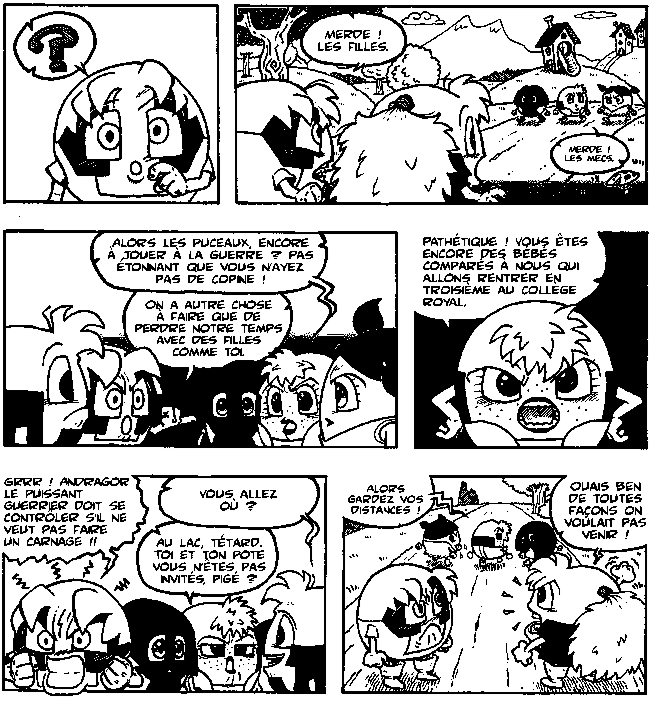
\includegraphics[trim= 0mm 0mm 0mm 0mm, clip, width=0.3\textwidth]{binary.png}}	\hspace{2em}
		\subfloat[Connected-component bounding boxes]{\label{fig:pe:cc_bounding_box}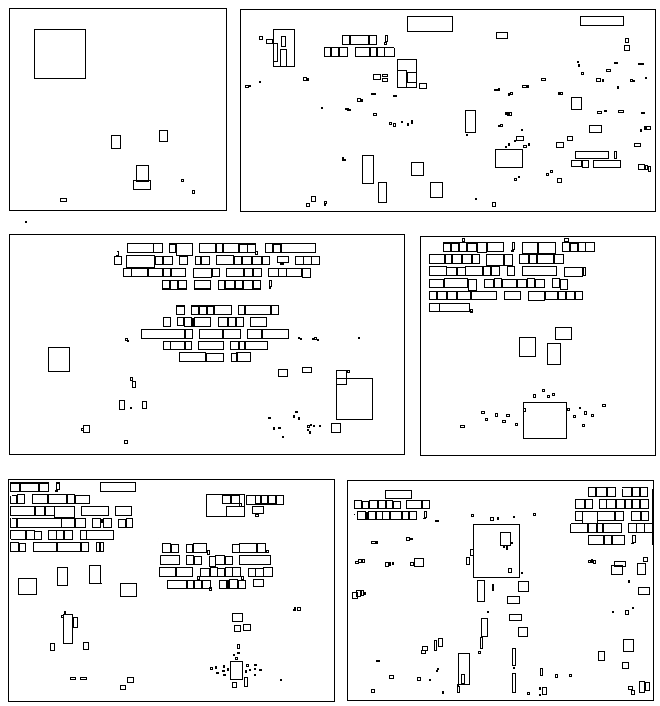
\includegraphics[trim= 0mm 0mm 0mm 0mm, clip, width=0.3\textwidth]{roi.png}}
		\\
		\subfloat[Panels from k-means classification]{\label{fig:pe:frame_unrecognized}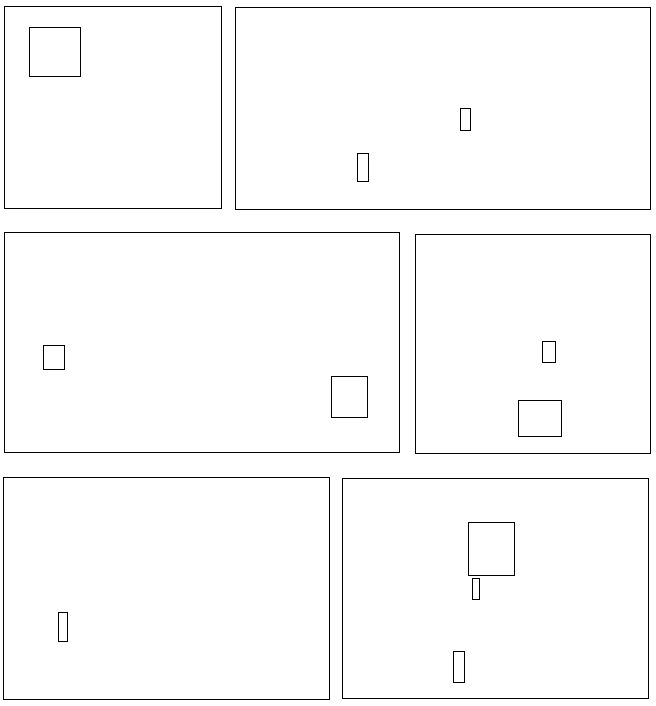
\includegraphics[trim= 1mm 0mm 0mm 0mm, clip, width=0.3\textwidth]{frame_unrecognized.png}}	\hspace{2em}
		\subfloat[Panels after topological filtering]{\label{fig:pe:frame_cleaned}
\includegraphics[trim= 1mm 0mm 0mm 0mm, clip, width=0.3\textwidth]{frame_cleaned.png}}
		  \caption{Panel extraction process. Image credits:~\cite{Bubble09}.}
		  %\label{fig:apl_1_0}
	\end{figure}
	%%%%%%%%%%%%%%%%%%%%%%%%%%%%%%%%%%%%%%%%%%%%%%%%%%%
% paragraph process (end)

\paragraph{Clustering} % (fold)
\label{par:clustering}
By looking at the figure~\ref{fig:pe:cc_bounding_box}, we can clearly see that the bounding boxes of the panel are bigger than the others.
Also, their includes more regions than others.
Classifying those regions according to their size would allow us to classify panel but also text region at the same time.
Knowing the number of classes helps a lot in classifying data, here 
% The classification of connected-component heights using k-means algorithm. 
%We define the set of component bounding boxes $R = \{R_1, R_2, ... , R_n\}$.
we define three classes according to the domain knowledge of comics.
The three classes corresponds to ``panel'' (the highest), ``text'' (the most numerous) and ``noise'' (few pixels height) as shown on figure~\ref{fig:pe:histo_roi}.
One of the most popular clustering algorithm is k-means clustering method.
It aims to partition $(x_1, x_2, ...,x_n)$ observations into $k$ clusters ($k <= n$) $S=\{S_1, S_2, ..., S_k\}$ in which each observation belongs to the cluster with the nearest mean.
This optimisation problem is formulated as formula~\ref{eq:pe:k-means}.

\begin{equation}
	arg min \sum\limits_{i=1}^k \sum\limits_{n_j \in S_i} ||x_j - \mu_i||^2
	\label{eq:pe:k-means}
\end{equation}
where $\mu_i$ is the mean of points in the cluster $S_i$.

This clustering is performed dynamically on each image which makes this method invariant to page format and resolution.
% Indeed, the height-based classification is not page size dependent unlike~\cite{Khoi11,Arai11}, and the number of pixels for each ROI is proportional to the page resolution (do not bias the classification).

	%%%%%%%%%%%%%%%%%%%%%%%%%%%%%%%%%%%%%%%%%%%%%%%%%%%
	\begin{figure}[!ht]	%trim=l b r t  width=0.5\textwidth, 
	  \centering
		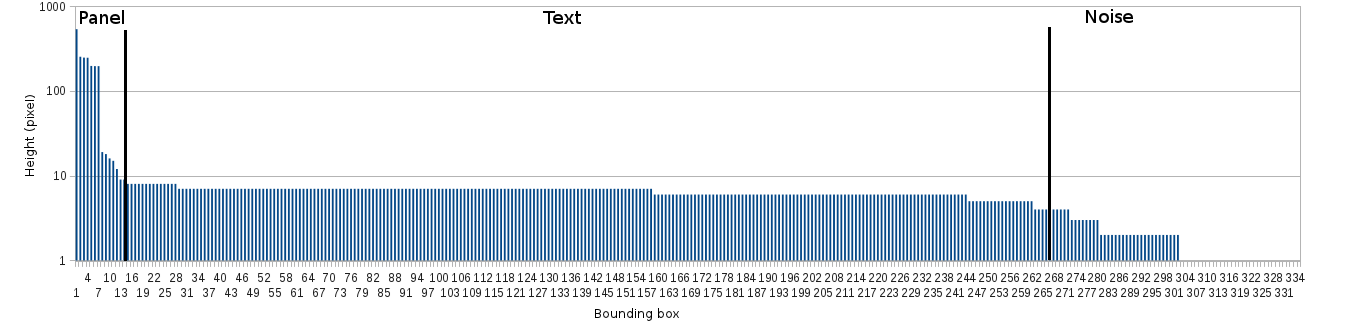
\includegraphics[height=27mm]{Histogram_en.png}
		\caption{Descendent histogram of the bounding boxes of figure~\ref{fig:pe:cc_bounding_box}. Vertical black lines represent an example of three classes separation.}
		\label{fig:pe:histo_roi}
	\end{figure}
	%%%%%%%%%%%%%%%%%%%%%%%%%%%%%%%%%%%%%%%%%%%%%%%%%%%

\paragraph{Topological filtering} % (fold)
\label{par:topological_filtering}
After the classification step, the second characteristic of panel is used in order to keep only the components that are not overlapped by others.
We define the set of component bounding boxes $R = \{R_1, R_2, ... , R_n\}$ and filter out components that do not verify this relation $R_i\notin{R_j} \forall j, i \neq j$.
See figure \ref{fig:pe:frame_unrecognized} and~\ref{fig:pe:frame_cleaned}.

	%%%%%%%%%%%%%%%%%%%%%%%%%%%%%%%%%%%%%%%%%%%%%%%%%%%
	% \begin{figure}	%trim=l b r t  width=0.5\textwidth, 
	%   \centering
	% 	%\includegraphics[height=60mm]{figure/BUBBLEGOM_T01_P007_crop.jpg}
	% 	%\includegraphics[trim= 0mm 0mm 0mm 0mm]{figure/BUBBLEGOM_T01_P007.jpg}
	% 	\subfloat[Frame from k-means clustering]{\label{fig:frame_unrecognized}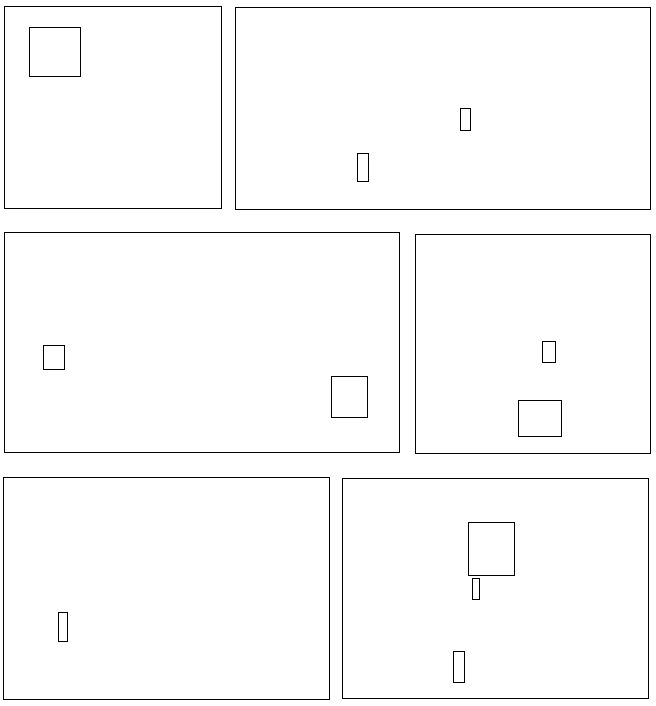
\includegraphics[trim= 1mm 0mm 0mm 0mm, clip, width=0.30\textwidth]{frame_unrecognized.png}}	\hspace{2em}
	% 	\subfloat[Frame after topological filter]{\label{fig:frame_cleaned}
\includegraphics[trim= 1mm 0mm 0mm 0mm, clip, width=0.30\textwidth]{frame_cleaned.png}}
	% 	  \caption{Topological filtering of the frames}
	% 	  %\label{fig:apl_1_0}
	% \end{figure}
	%%%%%%%%%%%%%%%%%%%%%%%%%%%%%%%%%%%%%%%%%%%%%%%%%%%
% paragraph topological_filtering (end)

% paragraph classification (end)

% subsection k_mean_classification (end)



\subsection{Outermost contour analysis} % (fold)
\label{sub:outermost_contour_filtering}
The previous clustering-based method is particularly useful for multi component extraction, for instance if we want to extract panel and text at the same time.
Nevertheless, for panel only extraction we can improve the method by using the second characteristic of panels which is in their topological relations with the other connected-components.
Figure~\ref{fig:pe:cc_bounding_box} shows that outermost (external) contours actually corresponds to panels.
This is especially true for general comics using gutter (white space) between panels.
% We propose to combine the advantages of the already published panel extraction methods~\cite{Arai11,Rigaud2012LNCS} and partially solve their weaknesses using the expert system model.
% that we present section~\ref{sec:expert_system}.
% They are connected component based methods that are reliable for comics with disconnected panels (separated by gutters).
% no gutter between the panels (they are separated by a single black line).
% Line-based decomposition methods are the efficient methods for line separated comics~\cite{Li2013Unsupervised} (no gutter).
% A generic method that works best with both styles is not obvious.
% We combine~\cite{Arai11,Rigaud2012LNCS} to introduce a new method, especially suitable for general comics using gutter (white space) between panels.
Here we also improve the binary image segmentation using adaptive thresholding method.
Adaptive thresholding consist in deciding if a pixel at position $(x,y)$ belongs to the foreground or background according to the mean value of its neighbourhood pixels in a window of size $blockSize * blockSize$.
% r each pixel position $T(x,y)$ is a mean of the $blockSize * blockSize$ neighbourhood of point of coordinates $x,y$.
The $blockSize$ is an odd value related to the image size as defined by equation~\ref{eq:panel_blockSize}.
Note, we add one if the result is not odd in order to make sure the point $(x,y)$ is at the centre the region.

\begin{equation}
\label{eq:panel_blockSize}
	blockSize = \frac{I_{width} + I_{height}}{2} * blockSizeFactor
\end{equation}
where $blockSizeFactor$ corresponds to a constant discussed section~\ref{sec:eval_panel}. 
A minimum area is also required to be considered as a panel $minAreaFactor$ to avoid considering surrounding elements as panel.
% area of size  in order to be contrast invariant.
% External (or outermost) contours are the contours that are not included in other contour, see figure~\ref{fig:panel}.
% See the evaluation of the method section~\ref{sec:eval_panel}.


%%%%%%%%%%%%%%%%%%%%%%%%%%%%%%%%%%%%%%%%%%%%%%%%%%%
 % \begin{figure}[!ht]  %trim=l b r t  width=0.5\textwidth,
 %   \centering
 %  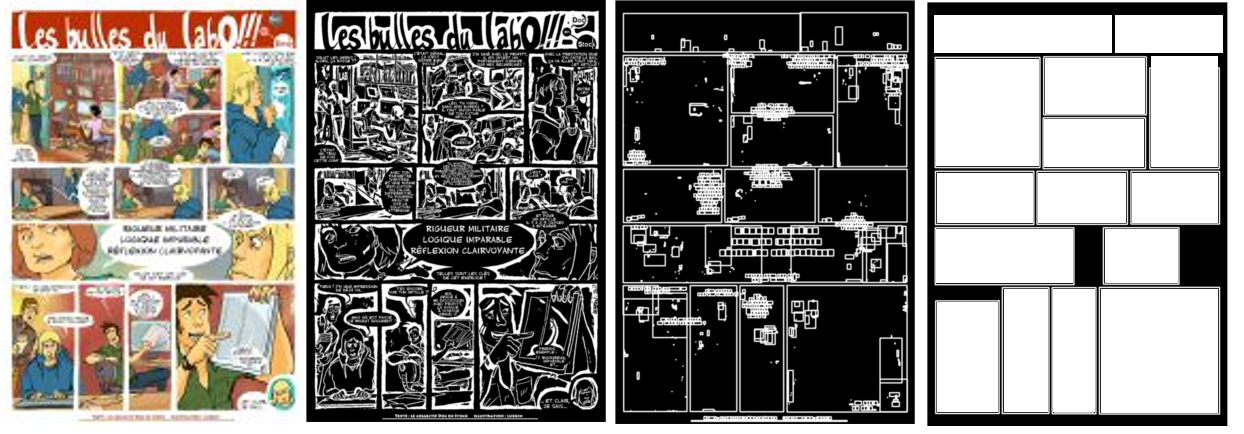
\includegraphics[width=240px]{panel_detection.png}
 %  \caption{Contour detection and filtering of panel.
 %  Original image, adaptive thresholding, contour bounding boxes and results mask of the outermost contours from left to right.}
 %  \label{fig:panel}
 % \end{figure}
%%%%%%%%%%%%%%%%%%%%%%%%%%%%%%%%%%%%%%%%%%%%%%%%%%%

% subsection outermost_contour_filtering (end)

% Experiments --------------------------------------------------------------------------------------------------------
\section{Experimental results}
\label{sec:pe:experimental_results}
We evaluated the proposed method on the 850 panels of the eBDtheque dataset~\cite{Guerin2013} ``version 2014'' at bounding box level.
% with $th_0=0.5$. % according to equation~\ref{eq:recall} and~\ref{eq:precision}.
In this experiment we set $blockSizeFactor = 1\%$ according to the validation on the eBDtheque dataset~\cite{Guerin2013} table~\ref{tab:blockSizeFactor_validation}.
Note, we could also choose $blockSizeFactor = 5\%$ which has a slightly better performance but it is two times slower.
 

%%%%%%%%%%%%%%%%%%%%%%%%%%%%%%%%%%%%%%%%%%%%%%%%%%%
  \begin{table}[ht]
    % \normalsize
    \centering
    \caption{Validation of the parameter $blockSizeFactor$ on the f-measure $F$ and the average processing time $t$ per panel.}
    \begin{tabular}{|c|c|c|}
		\hline
		$blockSizeFactor$ (\%) & $F$ (\%) 	&$t$ (s)\\
		\hline 
		10 & 83.22 & 0.22 \\
		\hline
		5 & 84.25 & 0.10 \\
		\hline
		4 & 83.0 & 0.07 \\ 
		\hline
		3 & 83.06 & 0.05 \\
		\hline
		2 & 75.79 & 0.04 \\ 
		\hline
		\textbf{1} & \textbf{84.12} & \textbf{0.05} \\
		\hline
		0.5 & 82.0 & 0.06 \\
		\hline

	\end{tabular}
    \label{tab:blockSizeFactor_validation}
  \end{table}%
%%%%%%%%%%%%%%%%%%%%%%%%%%%%%%%%%%%%%%%%%%%%%%%%%%%

Assuming that a panel is a big region, we ignored the panel detection with a area lower than 4\% ($minAreaFactor$) of the page area according to the parameter validation on the eBDtheque dataset table~\ref{tab:minAreaFactor_validation}.


%%%%%%%%%%%%%%%%%%%%%%%%%%%%%%%%%%%%%%%%%%%%%%%%%%%
  \begin{table}[ht]
    % \normalsize
    \centering
    \caption{Validation of the parameter $minAreaFactor$ on the f-measure $F$ and the average processing time $t$ per panel.}
    \begin{tabular}{|c|c|c|}
		\hline
		$minAreaFactor$ (\%) & $F$ (\%) 	&$t$ (s)\\
		\hline 
		10 & 62.97 & 0.13 \\
		\hline
		8 & 71.43 & 0.10 \\
		\hline
		6 & 77.0 & 0.07	\\
		\hline
		\textbf{4} & \textbf{83.81} & \textbf{0.05} \\
		\hline
		2 & 82.75 & 0.04 \\
		\hline
		% \textbf{1} & \textbf{84.12} & \textbf{0.05} \\
		% \hline
		1 & 76.0 & 0.03 \\
		\hline

	\end{tabular}
    \label{tab:minAreaFactor_validation}
  \end{table}%
%%%%%%%%%%%%%%%%%%%%%%%%%%%%%%%%%%%%%%%%%%%%%%%%%%%


%Those heuristics have been chosen very large to filter out aberrant regions such as very small region and page border.

Table~\ref{tab:panel} presents the average results we obtained compared to the cluster-based method presented in section~\ref{sub:k_mean_clustering} and a method from the literature~\cite{Arai11}.

    %%%%%%%%%%%%%%%%%%%%%%%%%%%%%%%%%%%%%%%%%%%%%%%%%%%
  \begin{table}[ht]
    \normalsize
%\renewcommand{\arraystretch}{1.2}

    \centering
    \caption{Panel extraction results.}
    \begin{tabular}{|c|c|c|c|}
          % \hline
          %   & \multicolumn{2}{|c|}{Character 1}   & \multicolumn{2}{|c|}{Character 2}   \\
          \hline
          &  $R$ (\%)  & $P$ (\%)  & $F$ (\%)     \\
          \hline
          Arai~\cite{Arai11}   & \modif{58.03}       & \modif{75.30}    & \modif{65.55}    \\
          \hline
          Method 1   & 78.02       & 73.17   & 75.52     \\
          \hline
          Method 2   & 81.24     & 86.55     & 83.81      \\
          \hline
           % TOTAL   & 93.4    & 92.8          \\
          % \hline
        %       Proposed multi scale & ???  &???  & ???   & ???       \\
        %   \hline
        \end{tabular}
    \label{tab:panel}
  \end{table}%
    %%%%%%%%%%%%%%%%%%%%%%%%%%%%%%%%%%%%%%%%%%%%%%%%%%%

% {\bf ADD} analysis here.
% What type of comic book works best/worst, advantage/disavantage, see appendix~\ref{ap:Panel_object_proposed}

\begin{figure*}
 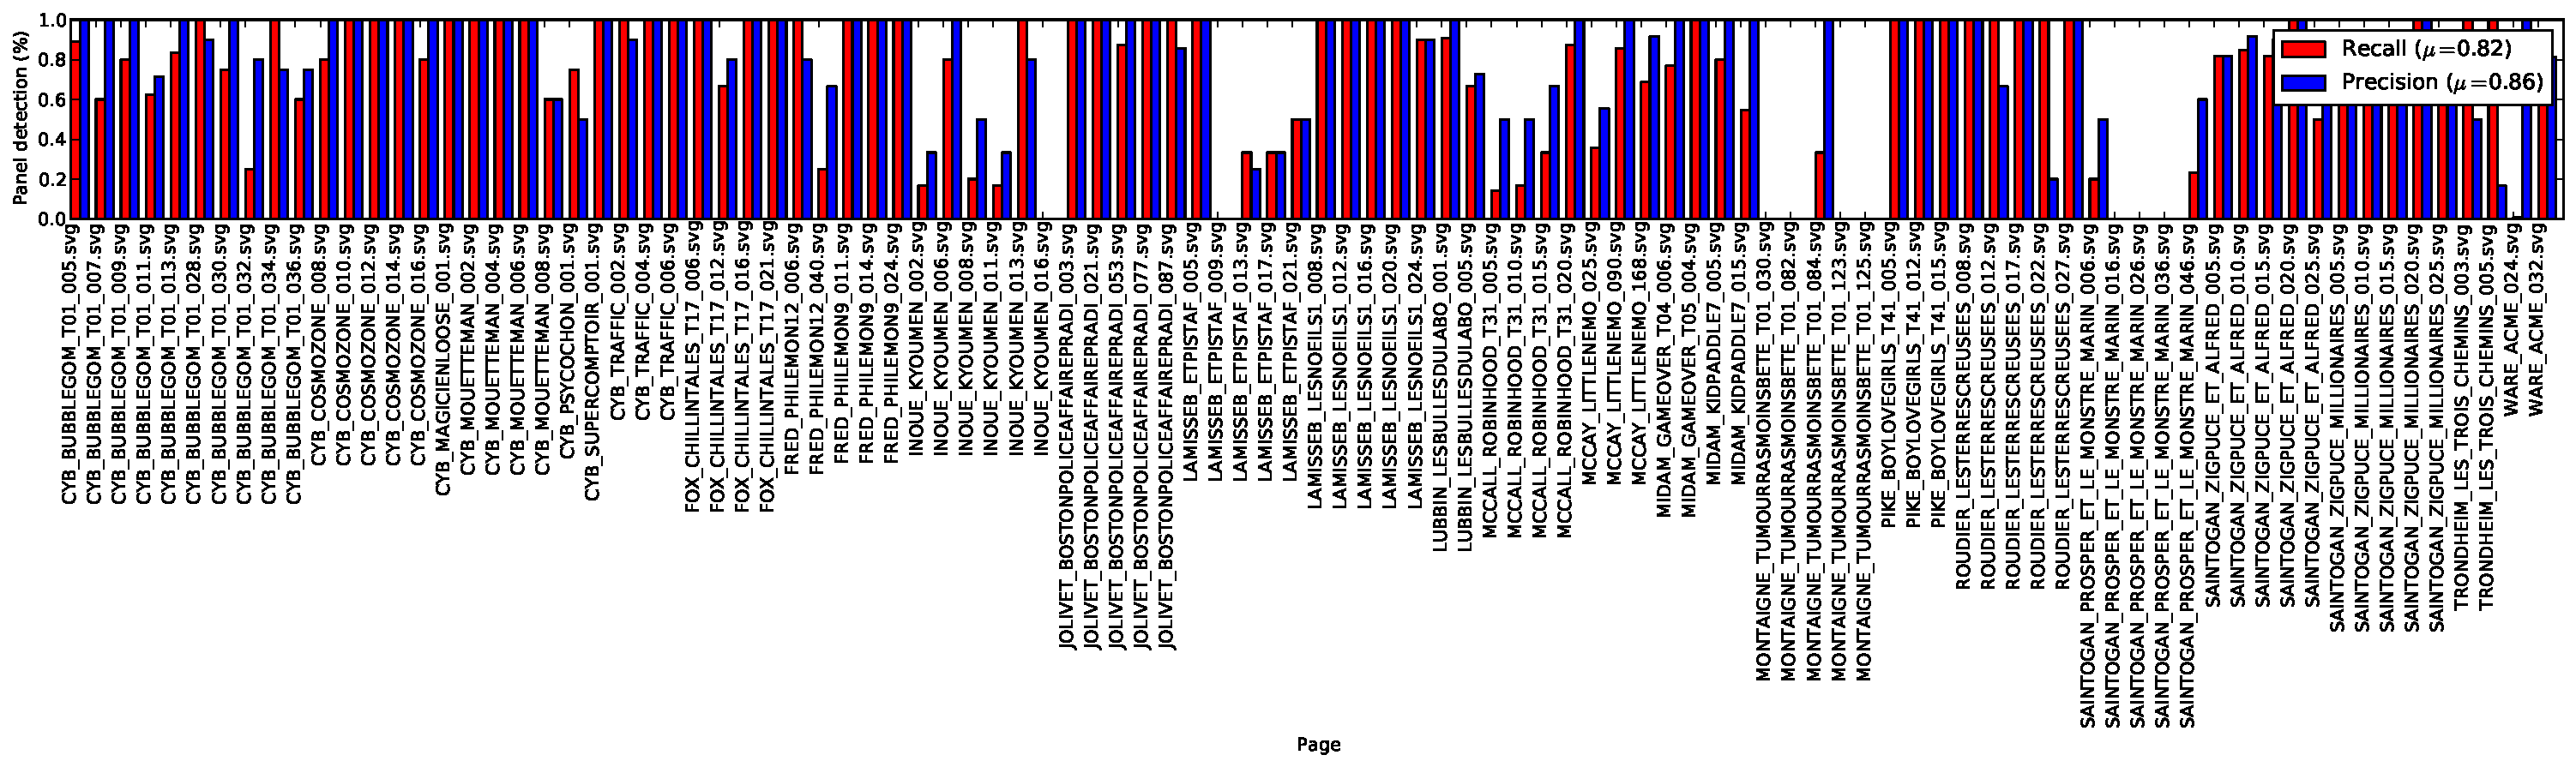
\includegraphics[width=\textwidth,height=4cm]{Panel_object_proposed.pdf}
 \caption{Panel extraction score details for each image of proposed topological approach on the eBDtheque dataset~\cite{Guerin2013}
 }
 \label{fig:pe:panel_extraction_ijdar}
\end{figure*}

\begin{figure*}
 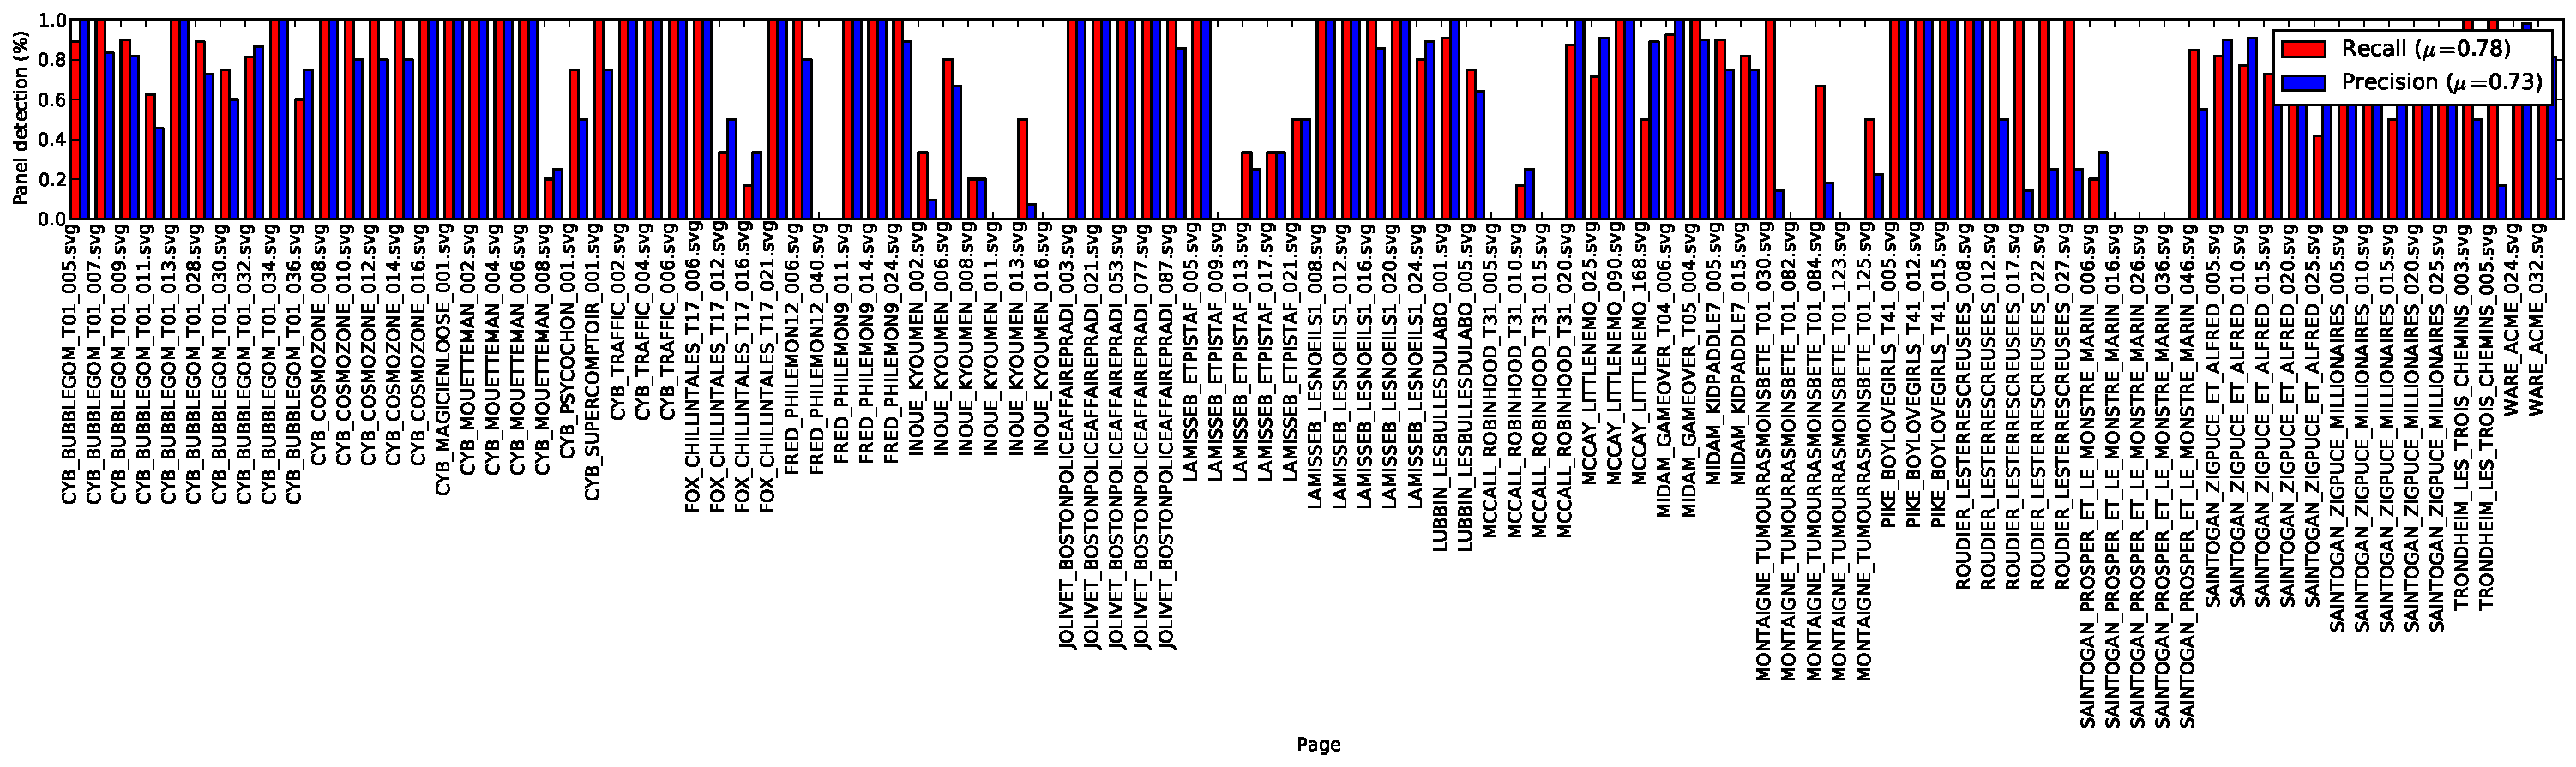
\includegraphics[width=\textwidth,height=4cm]{Panel_object_Rigaud_CIFED_2012.pdf}
 \caption{Panel extraction score details of the proposed k-means based method for each image of the eBDtheque dataset~\cite{Guerin2013}
 }
 \label{}
\end{figure*}

The proposed panel extraction based on connected component analysis is a simple to implement, fast and efficient method for comics with disconnected panels (separated by a white gutter).
Figure~\ref{fig:pe::panel_extraction_lncs} and \ref{fig:pe:panel_extraction_ijdar} show the details for each tested image for the two proposed methods.
The proposed methods are not appropriate for gutter-less comics such as ``INOUE'' or strip without panel border such as ``MONTAIGNE'' or a extra frame around several panels (``SAINTOGAN\_PROSPER'').
Another weakness occurs when panels are connected by other elements due to the limitations of the connected-components labelling method.
This experiment was performed in 28 seconds for the whole dataset using one CPU at 2.5GHz (0.05s per panel in average).
Note, pages of ``SAINTOGAN\_PROSPER'' are double pages that have been digitized with a dark background surrounding the cover. This is a noise due to the digitization process that we automatically remove by cropping image where a panel with an area $>$ 90\% of the page area is detected.

% Conclusion --------------------------------------------------------------------------------------------------------------------------------------
\section{Conclusions}
\label{sec:pe:conclusion}

Both methods have been published in ~\cite{Rigaud2012LNCS} and [pending acceptance???].

% K-mean classification

This method assumes that the page contains text with background brightness similar to page background otherwise the binary segmentation process and thus the classification may fail.

Then, the variance of each class is computed to check the homogeneity of the ROI. If the variance of the ``frame'' class is high, a specific algorithm~\cite{Khoi11} is applied in order to improve the previous steps (binarisation and/or classification). 
